\section{Classification methods}
Using the generated features 4 methods are applied to classify the data between happy tweets and sad ones. The three first are classic feature classifications that were applied to the tweets features. The last one is a more complex classification method and is directly applied on the embeddings.

\subsection{Logistic regression}
The first classifier that is applied is standard logistic regression. This classifier use the logistic function to determines whether the tweets belongs to one categories or another. This really simple method as the advantage that it is really fast to compute and easy to implement. It can be use to determine if the modification of the data processing as an impact on classification. But it will not be efficient enough to use for the competitions.

\subsection{SVM}
The more advanced classification technic of \textit{Support vector machine} is implemented as well. This method is often use in supervised learning. Given a set of training example belonging to two different categories, the SVM model build a frontier between the samples of the two categories with the biggest gap possible. This technics leads to better results for classification but also takes more times to run. 

\begin{figure}[h!]
\centering
	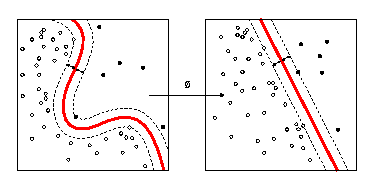
\includegraphics[scale=1.2]{SVM} 
\caption{The SVM model tries to find the frontier with the bigger gap possible.}
\label{plot:SVM}
\end{figure}
\FloatBarrier

\subsection{Regular neural networks}

Neural nets were also used on tweets features. This neural net has one layers of size (200,100) . This was to take account that a neural network of  two layers is sufficient to represent any vectorial function.  If this technic was giving the best results of all the one that were used on on tweets representation, it didn't lead to the sufficiently good results for the competition. 

\subsection{Convolutional neural networks}

In order to achieve better classification, a convolutional neural network is applied. The idea is not just to look as the tweet as a vectorial sum of embeddings, but to consider their places in the tweets as well. In this case, all the tweets are represented by a matrix :  At each word of the tweet corresponds a line of the matrix, containing the embeddings of the words. This matrix has therefore a size of \texttt{(number of words in the tweet * dimension of embeddings)}. A first layer apply then the convolution, it creates some filters of given sizes (in this case  3,4,5), which will be slided over the tweets matrix and output a results according to an activation function (in this case relu). Each convolution will create a tensor of a different size. A pooling process is then applied to theses different tensors, this will subsample the different tensors into tensors of a standard shape. Theses tensors are then combined to create a big feature vector of size \texttt{(batch size * total number of filter)}. These features are then use to get the prediction using matrix multiplication. 

\subsection{Dropout layer}
A classical problem in machine learning is overfitting. When a fully connected convolutional neural network is trained, allowing all the nodes to interact between them allows to much freedom for the system and it will overfit the data. To reduce this problem, a ``dropout'' is added to the convolutional neural network. At each step of the process a node is either kept or dropped out of the model with a given probability.  Of course the input nodes are excluded of this procedure in order to keep the most information. When data are tested, the full net is used and all the nodes are weighted by the keeping probability. 

This methods has two big advantages : first, as all nodes are not trained with all the data, overfitting will be reduced. Second, the method improves significantly the speed of training. This technic reduces nodes interactions too, and therefore it leads to more robust features.

\begin{figure}[h!]
\centering
	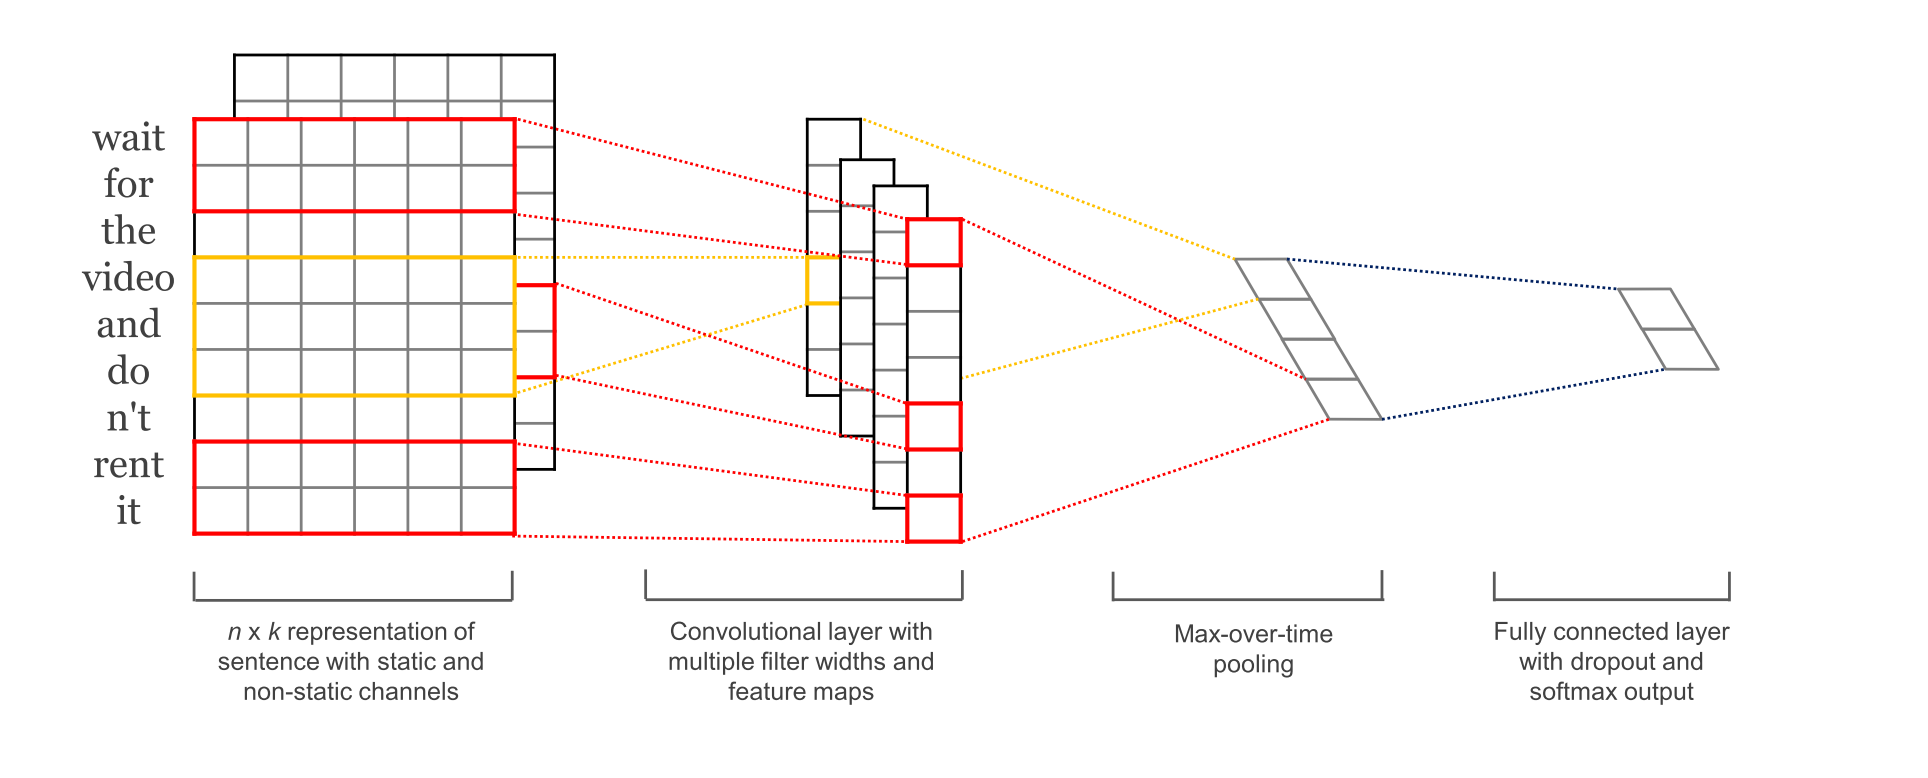
\includegraphics[scale=0.3]{CNN} 
\caption{Model of the convolutional neural network used for sentiment analysis}
\label{plot:CNN}
\end{figure}
\FloatBarrier
\label{sec:methods}
